Mellan 2017 och 2018 ökade säkerhetsbranschen med cirka 8 procent och omsatte 39 miljarder kronor i Sverige.
Detta beror inte på att brottsligheten ökar, utan på att fler svenskar upplever att brottsligheten ökar,
menar Jerzy Sarnecki, professor i kriminologi\cite{sverigesRadio}. För att fler svenskar ska uppleva en förhöjd känsla av säkerhet behöver ett tryggt och användarvänligt larmsystem etableras på marknaden.

\subsection{Syfte}

Projektet syftar till att utveckla och konstruera ett larmsystem
som bidrar till att fler svenskar upplever en förhöjd känsla av säkerhet i sina hem.

\subsection{Mål}

Målet med projektet är att utveckla ett larmsystem med hjälp av en mikrokontroller och ett antal periferienheter.
Larmsystemet, som består av ett grundsystem med ett antal tilläggsfunktioner, är effektivt och användarvänligt.

Grundsystemet utgörs av en centralenhet, en dörrlarmsenhet (periferienhet 1), en rörelselarmsenhet (periferienhet 2) samt en störenhet. Inställningarna för de två periferienheterna kan konfigureras via centralenheten.

Tilläggsfunktionerna delas in i två delar: (1) viktiga funktioner och (2) mindre viktiga funktioner. De viktiga funktionerna omfattar en funktion att slå om från produktionsläge till testläge för enklare test av periferienheterna samt en funktion som gör systemet självlärande.  De mindre viktiga funktionerna omfattar    kryptering av meddelanden som skickas i systemet samt framtagandet av en uppseendeväckande larmsignal.

\subsection{Arbetsmetod}

Som grund för arbetet med projektet ligger en tidsplan och ett antal milstolpar som tagits fram vid projektets uppstart. För att kontinuerligt stämma av hur väl projektets delmål uppnås sker regelbundna möten där samtliga gruppmedlemmar förväntas deltaga. Vid behov kan resurser omfördelas för att nå projektets delmål.

Tidsplanen är ingen detaljplanering, utan en överblicksplanering, som används för att fördela resurser inför den kommande veckan. Detta är fördelaktigt då det kan vara svårt att detaljplanera hur arbetet ska utföras innan det är kännt vilka förutsättningar som råder när arbetet ska utföras.

\subsubsection{Versionshantering}
För projektet har versionshanteringssystemet \textit{Git} använts. All kod finns tillgänglig på ett fjärrarkiv på \textit{GitHub}.

\subsubsection{Dokumentation}

Projektet är dokumenterat genom möteskallelser och -protokoll samt genom att använda \textit{Issue}-funktionen på GitHub. För buggrapportering, frågor och återkoppling om dokumentation eller kod, samt granskning av testfall, öppnas ett ärende (\textit{eng.} issue) på GitHub. Diskussionen kring ett ärende sker i ärendets kommentarsfält. Samtliga öppna ärenden tas upp på veckomötena där de diskuteras och nästa steg bestäms. Det som diskuteras på ett veckomöte dokumenteras sedan i ärendets kommentarsfält. Genom att samla alla projektets problem (buggar) och frågor på samma ställe kan samtliga gruppmedlemmar och kunden få en övergripande bild av vad som inte fungerar, vart projektet är på väg och vad som måste göra. 

\subsubsection{Mjukvaruutveckling och testning}

Under projektet implementeras de krav som kunden ställt på grundsystemet (se tabell \ref{tabell:krav} på sida \pageref{tabell:krav}). För att kontrollera att kraven uppnås - och därmed kvalitetssäkra produkten - skrivs och utförs ett testfall för varje krav. Om det körda testet blir godkänt är kravet uppnått.

Under mjukvaruutvecklingen integreras utveckling med testning för att kunna leverera en högkvalitativ produkt. För att så tidigt som möjligt i utvecklingsfasen hitta och lösa buggar testas en funktion (ej att förväxla med krav) så fort den har utvecklats. Dessa tester utförs i första hand i hårdvaran, men vid behov används en simulator. Fördelen med att testa direkt i hårdvaran är att det som fungerar i en simulator inte nödvändigtvis behöver fungera i hårdvaran, vilket skapar ett extra teststeg.

\subsubsection*{Funktionella tester och användartester}

I projektet utförs funktionella tester som testar funktionaliteten av olika delar av systemet, prestandatester för att fastställa systemets prestanda och kapacitet, samt användartester för att upptäcka förbättringar av systemet utifrån ett användarperspektiv. Varje testfall består av följande data:

\begin{description}
  \item [ID] Ett unikt ID på formen TXnnnvm, där X är F, P eller A för funktionellt test, prestandatest respektive användartest, nnn är ett nummer mellan 0 och 999 tilldelat i den ordning testfallen skapats, och m är versionsnummret. Exempelvis är TF012v3 den tredje versionen av det tolfte funktionella testfallet.
  \item [Namn] Ett namn som tydligt beskriver vad testfallet ska testa.
  \item [Beskrivining] En beskrivning av testfallet. Beskrivningen ska beskriva syftet med testfallet, vilken komponent som testas, vilket eller vilka krav som testas samt eventuella tekniska förutsättningar för att genomföra testet.
  \item [Teststeg] De steg som måste utföras för att utföra testfallet.
  \item [Förväntat resultat] Beskrivning av det förväntade resultatet för testfallet.
\end{description}

\noindent
Eftersom produkten kvalitetssäkras av tester är det självklart viktigt att kvalitén på testfallen och utförandet av dem är mycket hög. För att säkerställa att alla testfall som skrivs håller en hög kvalité sker skapandet och utförandet av testfallen enligt följande rutin:

\begin{enumerate}
\item När ett testfall skapas tilldelas det automatiskt status \textit{Utkast}. Testfallet kan sedan skickas vidare till \textit{granskning}.
\item Granskningen ska ske av åtminstone en (1) person och personen får inte ha varit inblandad i skrivandet av testfallet. Testfallet kan antingen bli \textit{godkänt} eller \textit{avfärdat}.
\item Om testfallet blir godkänt ändras dess status till \textit{Klar för test} och det får köras. Om testfallet däremot blir avfärdat måste det revideras och sedan åter skickas till granskning.
\item Ett föråldrat eller inaktuellt testfall med status \textit{Klar för test} kan skickas tillbaka till granskning.
\end{enumerate}

\noindent
Denna rutin visualiseras i figur 1.

De två reglerna för att skapa och köra testfall är följande: (1) endast testfall med status \textit{Utkast} får redigeras och (2) endast testfall som har blivit granskade och godkända får köras.

\begin{figure}[h]
  \centering
  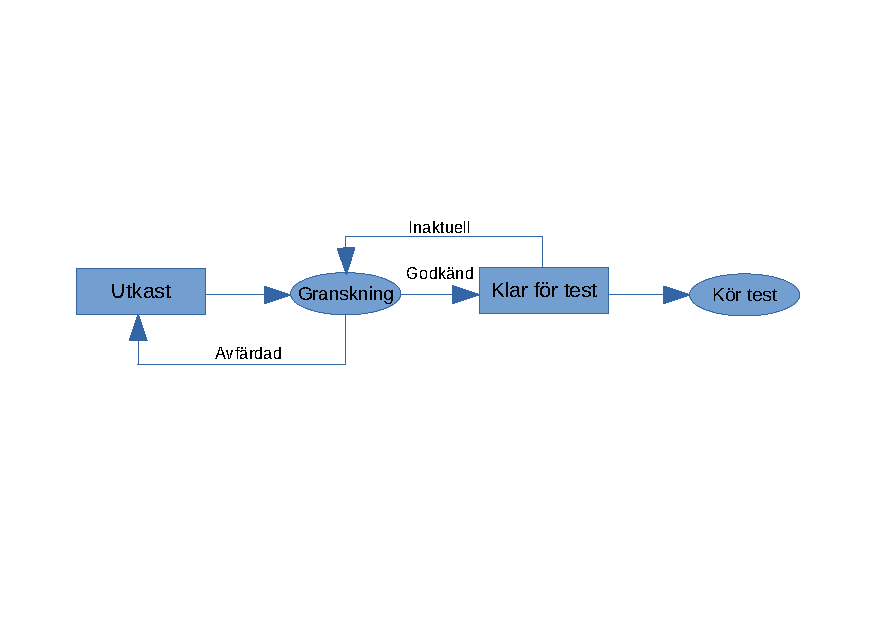
\includegraphics[trim={0 4cm 0 3cm}, clip, scale=0.8]{figurer/testrutin.pdf}
  \caption{Rutin kring att skriva och genomföra testfall.}
\end{figure}

\noindent
Samtliga körda testfall är samanställda i appendix A och resultatet av samtliga körda tester är sammanställda i appendix B.

